\newcommand{\HRK}{\emph{Hello rootKitty}}

\chapter{Hypervisor-enForced Execution of Security-Critical Code}\label{hyperforce}

\epigraph{2in}{La semplicit\'a \'e l'estrema perfezione (Simplicity is the ultimate sophistication)}{Leonardo da Vinci}{}




Leveraging virtualisation technology to mitigate attacks to operating system kernels with a very low impact is a challenging task because of the high overhead caused by the context switch between the guest and the hypervisor. An important goal for any framework employing virtualisation as a security tool, is to guarantee the execution of critical code in the kernel-space of the virtualised operating system regardless of the state of the kernel, i.e. code that will run identically in both clean and compromised kernels.
%Designing a countermeasure that protects virtualized operating systems is considered a challenge not only because of the difficulty to modify the target system (due to the lack of sources or licenses) but also because a virtualized system is already affected by consistent overhead, by design.
%An important goal for any framework using virtualization as a security tool, is to guarantee the execution of critical code in the kernel-space of a virtualized operating system regardless of the state of the kernel, i.e. code that will run identically in both clean and compromised kernels.

By critical code we refer to code that, in general, monitors the state of the system and that it is desirable, mainly from a security point of view, to maintain its execution. Examples of such code include the integrity checking of sensitive kernel-level data structures that are usually abused by rootkits or the scanning of files and memory areas for known malware signatures, as in the case of common antivirus systems. 
Given our assumption of a kernel-level attacker, it is also needed to ensure the integrity of the critical code itself to protect it from malicious modifications which might compromise its efficacy or completely deactivate its operations.
As explained in Chapter \ref{hellorootkitty}, a way of achieving such a goal is to implement and execute security-critical code within the hypervisor. Alternative approaches monitor the target system from a separate virtual machine in order to take advantage of isolation between the hypervisor and any virtual machine as well as isolation among multiple virtual machines \cite{lares, outvm, livewire}.
Unfortunately, both approaches are known to be affected by a consistent performance overhead. Moreover, when integrity checking methods are considered, the amount of guest memory to be checked, in order to reduce the attack surface considerably, can impose an overhead or detection time that might prohibit the adoption of such solutions in production systems. 

Designing approaches in which guest operating systems cooperate with the hypervisor can lead to high degrees of security, even comparable to the ones guaranteed by completely isolated systems, while significantly reducing the overall performance impact.


\section{Problem description}
%TODO put motivation from paper and write it here.
% hypervisor-awareness usually reduces the performance impact but the lack of sources of the OS being virtualized (Windows) imposes the search of new strategies.
%The ``cloud'' is probably the most used technological term of the last years. Its supporters present it as a complete change in the way that companies operate that will help them scale on-demand without the hardware-shackles of the past. CPU-time, hard-disk space, bandwidth and complete virtual infrastructure can be bought at a moment's notice. Backups of data are synced to the cloud and in some extreme cases, all of a user's data may reside there (Chromium OS). Its opponents treat it as privacy nightmare that will take away the user's control over their own data and place it in the hands of corporations as well as a risk to the privacy, integrity and availability of user data~\cite{amazon_cloud_problem,exposingFHS2011}. Regardless however on one's view of the cloud, one of the  main technologies that makes the cloud-concept possible is virtualization.
%Virtualization is the set of technologies that together allow for the existence of more than one running operating systems on-top of a single physical machine. While initially all of the needed mechanisms for virtualization were created in software, the sustained popularity of virtualization, lead to their implementation in hardware, providing the desired speed that was lacking in their software counterparts. Today both Intel\footnote{\url{http://www.intel.com/technology/virtualization/technology.htm}} and AMD\footnote{\url{http://sites.amd.com/us/business/it-solutions/virtualization}} support a set of instructions that are there with the sole purpose of facilitating virtualization. Apart from the use of virtualization as way to host different operating systems on one machine, virtualization can also be used to provide greater security guarantees for operating systems. Researchers have already proposed various systems that use virtualization primitives that all fall in this category ~\cite{Criswell2007,Dewant2008,hellorootkitty,Gadaleta2009,Qubesos}. 
Despite the number of publications in the field of kernel level security (\cite{rootkitdetection, rootkitdetection2, HookSafe}), the consistent presence of kernel-level malware is a sign of how complicated kernel protection really is. 
Fortunately, virtualisation technology may facilitate the design of countermeasures that usually reveal to be effective. 

The chief difference between these systems that operate from within the hypervisor, (\textit{in-hypervisor}), and those that operate from within the target system, (\textit{in-guest}), is that the latter are part of the system's attack surface. Researchers have already proposed various systems that use virtualisation primitives that all fall in this category ~\cite{Criswell2007, Dewant2008, copilot, NICKLE, qubesos}.
%In general, current antivirus software that operates from within the same operating system to be protected, is one such system that could be deactivated or crippled by the attack itself. 

\textit{In-hypervisor} security systems, in contrast, can utilize the isolation guarantees of virtualisation technology to make sure that they will be active regardless of the state of the system that they protect. 
Unfortunately, these security benefits do not come for free. The constant transition from the virtualised operating system to the hypervisor (known as \texttt{VMExit}) and back (\texttt{VMEntry}), negatively affects the overall performance of the guest forcing one to choose between better security or better performance.

In this chapter we present a framework that facilitates the implementation of countermeasures to protect virtualised operating systems, with security and integrity comparable to those provided by \textit{in-hypervisor} systems but at the performance cost of \textit{in-guest} systems. The system described here follows a hybrid approach by maintaining the security-critical code within the guest, protecting its instructions and data and forcing its execution from the hypervisor. For the reasons explained above we called this framework \texttt{HyperForce}.

Taking advantage of the aforementioned framework, we re-implement the countermeasure described in Chapter \ref{hellorootkitty} since that functions as a typical \textit{in-hypervisor} rootkit-detection system. An evaluation of the countermeasure in \texttt{HyperForce} shows that it significantly outperforms the original version while maintaining comparable security guarantees.

The rest of the chapter is structured as follows. In Section~\ref{hf:approach} we explain the core idea of our approach followed by its design details. In Section~\ref{hf:evaluation} we evaluate the performance benefits introduced by this framework and measure its performance impact. Related work is discussed in Section~\ref{hf:related} and Section~\ref{hf:conclusion} concludes.

\section{Approach}\label{hf:approach}
The core idea of HyperForce is to combine the best features of the \textit{in-guest} and \textit{in-hypervisor} defence systems into a hybrid solution which performs as an \textit{in-guest} countermeasure while providing security comparable to \textit{in-hypervisor} countermeasures. 
We achieve this by deploying the functional part of the countermeasure within the guest operating system while maintaining its integrity and enforcing its execution with the assistance of the hypervisor. Since the functional part of the security-critical code, i.e. its instructions and data, is running within the virtualised operating system, the main advantage of such approach is that it has native access to the resources of the virtualised operating system such as the memory, disk and API of the virtualised kernel. 
This provides a great performance benefit for code that needs to access a high number of memory locations within the virtualised operating system since it alleviates the costly need of introspection usually required by in-hypervisor systems, i.e. the discovery of the corresponding physical memory pages of the guest's virtual memory pages and their remapping within hypervisor's space or another virtual machine's. 
%%Code executed from the same memory address space of the guest system is, on average, much faster than executing it from an isolated environment (such as the hypervisor or another virtual machine).  
%%We made a comparison between two monitoring approaches, one from hypervisor and one from the target system and provide details in Section \ref{casestudy}.

\paragraph{Enforcement of Execution.}
Given an arbitrary piece of security-critical code, HyperForce needs to ensure its execution at regular time intervals. A complete reliance for its execution on the virtualised operating system, could potentially allow a kernel-level attacker to intervene and inhibit the code's execution through the modification of the appropriate kernel-level data-structures. For instance, an attacker could locate the function pointer pointing to the security-critical code and overwrite it with a pointer towards their own code.

From a high-level view, HyperForce changes the execution flow of the guest kernel whenever the installed monitoring code has to be executed and restores the original execution flow upon code termination. 
The advances of virtualisation technology allows one to implement this transition in a multitude of ways. Our decision has been influenced by the desire of minimizing the amount of instrumentation code in the hypervisor and of keeping performance overhead to a minimum.

In our framework, the security-critical code is encapsulated within a function that is loaded in the virtualised operating system in the form of Loadable Kernel Module (LKM)\footnote{Although the proof-of-concept has been developed specifically for the Linux kernel, the method can be easily applied to other commodity operating systems such as Windows}. This allows the code to have native access to all of the guest operating system's resources.
The key component of HyperForce is a virtual device, created by the hypervisor's infrastructure, that is detected and treated as a regular hardware device by the guest operating system.  
%HyperForce then uses the infrastructure of the virtualization platform, specifically the Virtual Machine Monitor (VMM), to create a virtual device. 
Virtual devices are supported by all modern hypervisors to simulate real hardware, such as sound-cards, graphic cards, storage units, etc. and to allow the execution of unmodified guest code, as it has been designed to run on bare metal. 
Once the aforesaid virtual device has been created and loaded into the virtualised operating system, HyperForce registers the address of the memory location where the security-critical code has been stored to as an interrupt handler for the aforementioned virtual device. A schema is illustrated in Figure~\ref{hyperforce_schema}. 
The interrupt handler, and consequently the security-critical code, will be called whenever the virtual device generates an Non-Maskable Interrupt (NMI). Hence the cooperation of the hypervisor and the trusted module is based on this call-and-respond mechanism.
Since the virtual device is fully controlled by the hypervisor, it is the hypervisor that decides when interrupts must be generated and not the virtualised operating system. Due to this fact, the eventually compromised guest kernel has no possibility to anticipate or delay the execution of the security-critical code. The logic behind is hidden from it through the isolation mechanism guaranteed by virtualisation-enabled processors.  
This fact stops any attackers' efforts to evade detection by mimicking a non-compromised operating system just before the execution of the critical-code and restoring their malicious activities after it.

\begin{figure} 
\begin{center}
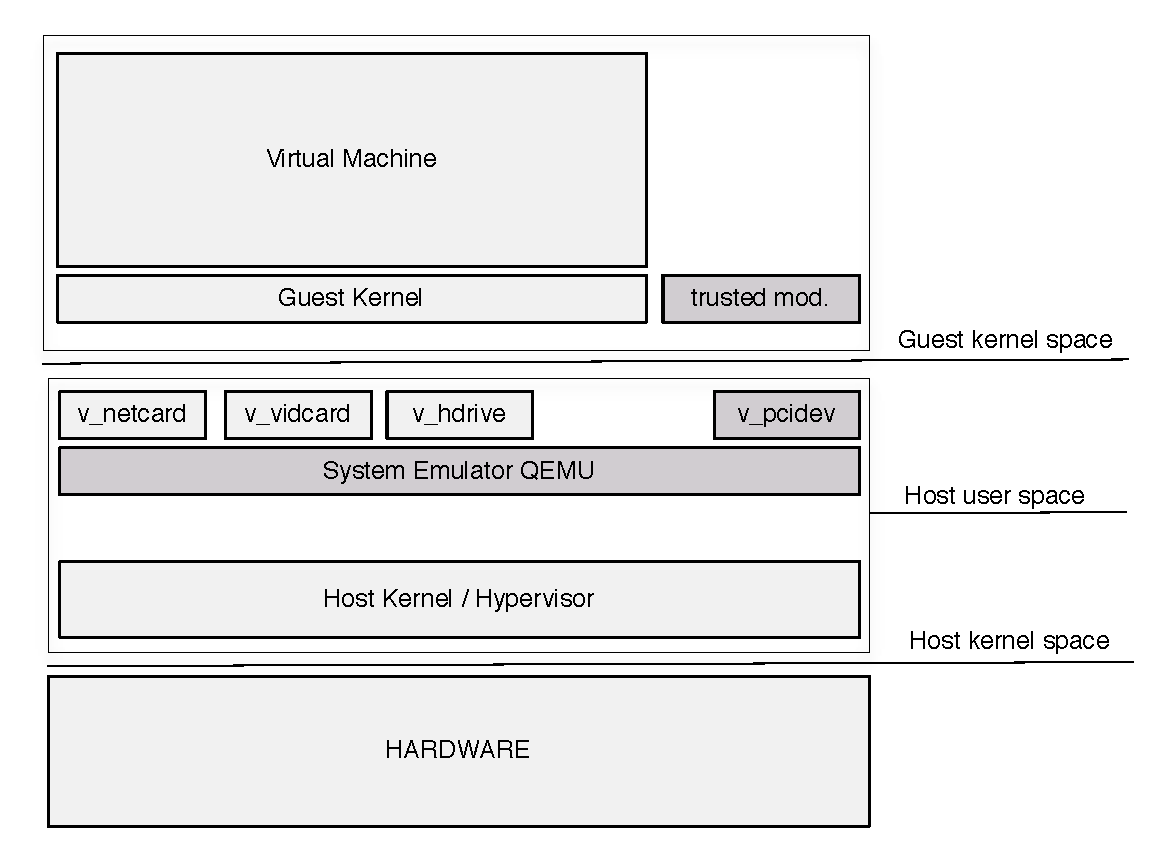
\includegraphics[scale=0.5]{images/hyperforce_schema.pdf}
\caption{Schema of HyperForce. Highlighted components indicate parts of the system that need instrumentation/modification}
\label{hyperforce_schema}
\end{center}
\end{figure}

\paragraph{Integrity of Code.}
%In the previous paragraph we described the loading of security-critical code within the hypervisor and the use of virtual devices to ensure the execution of that code.
Since the code is loaded in the guest as a LKM, it executes with the privileges of the virtualised kernel. While this is desired, it also opens up the code to attacks, e.g. modifications of its code and data, from an attacker who is in control of the virtualised kernel. 
Traditionally, the module could not be protected from the rest of the kernel since they both operate within the same protection ring, namely Ring 0. 
Due to virtualisation however, the hypervisor has more power than the virtualised operating system's kernel (signified as Ring -1) and can thus protect any resources from the virtualised kernel, including memory pages. 

HyperForce takes advantage of the paging system provided by the Linux kernel (extended with hypervisor capabilities) to write-protect the memory pages holding the instructions and data of the security-critical code. 
In order to allow the code to make changes to its data, HyperForce can unlock the memory pages before it triggers an interrupt of its virtual device and lock them back immediately after the code's execution. 
Most of the performance penalty is due to the task of trapping an access violation from the guest to the hypervisor. Hardware-supported extended page tables (Intel EPT or AMD NPT) for the memory management unit consistently reduces this performance impact.

Another way to circumvent the protection mechanism in place consists in compromising the Interrupt Descriptor Table (IDT), where pointers to interrupt handlers are stored. When an exploitable kernel-level vulnerability is found, it can be relatively easy to compromise the IDT. 
Therefore HyperForce write-protects the memory page holding the Interrupt Descriptor Table (IDT) of the protected guest. Lastly, HyperForce protects the Interrupt Descriptor Table Register (IDTR) that contains the address of the IDT, by checking its integrity at regular intervals. The aforementioned protection will prevent any attempt to use an Interrupt Descriptor Table that is different from the one observed within the untampered system.
The task of protecting the IDTR is a straightforward since the IDTR is not supposed to change during operating system lifetime. A schema of the selection of the interrupt gate via the IDTR is showed in Figure \ref{idtr}.

%In order to ensure that an attacker cannot avoid the execution of the interrupt handler containing the security-critical code, HyperForce also write-protects the memory page holding the Interrupt Descriptor Table (IDT) of the protected guest. Lastly, HyperForce protects the Interrupt Descriptor Table Register (IDTR) that contains the address of the IDT, as a regular invariant critical kernel object.


\begin{figure}
\begin{center}
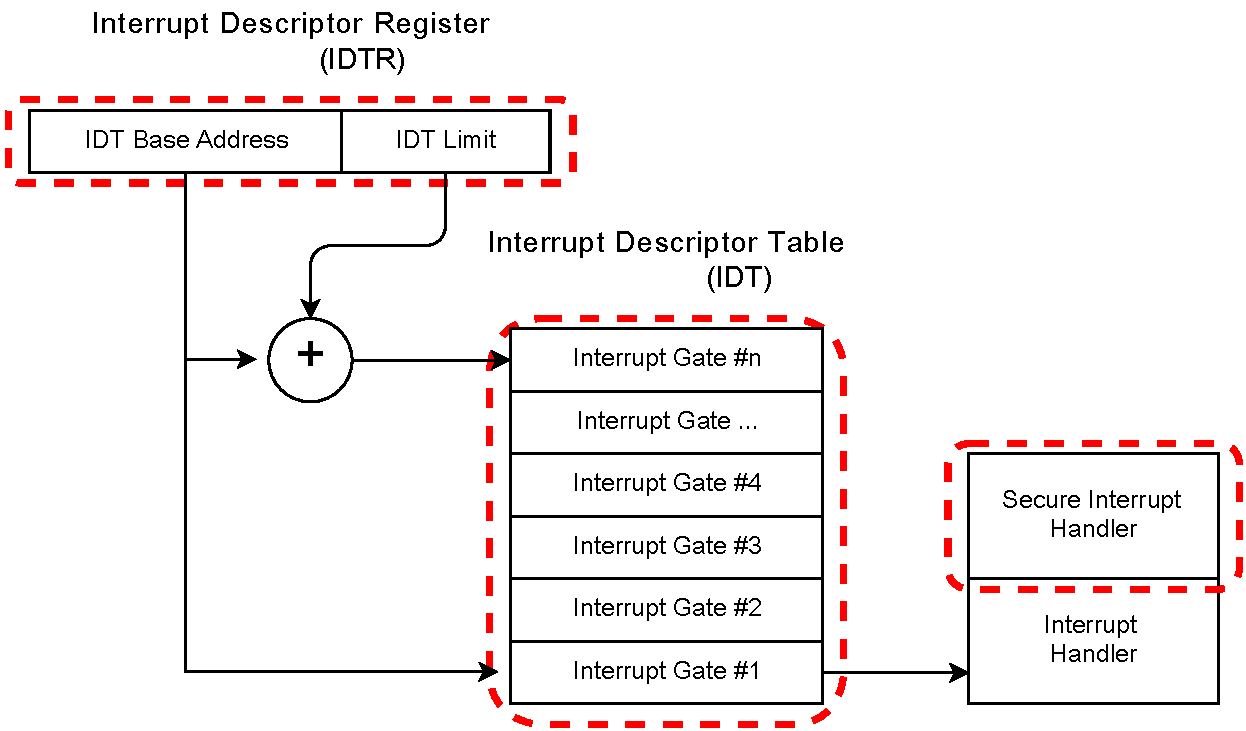
\includegraphics[scale=0.5]{images/IDTR.pdf}
\caption{Selection of Interrupt Gate via Interrupt Descriptor Table Register in the IA32 architecture. Dashed rectangles indicate that any attempt to write to these areas is trapped and handled by the hypervisor.}
\label{idtr}
\end{center}
\end{figure}


%
%\begin{comment}
%In order to guarantee complete isolation, modern hypervisors do not allow guest kernels to access and change the state of the hardware directly. To avoid this, system emulation is provided together with processor and memory virtualization.\\
%VMware [ref.] and QEMU/KVM \cite{qemu} are two widely deployed Virtual Machine Monitors - one commercial and one open source  - that provide full system hardware supported virtualization. Guest kernels will execute on an entirely virtualized system formed by virtual network cards, virtual hard drives, virtual video cards, etc.
%We implemented a proof of concept of HyperForce in QEMU/KVM because it is open source with an active community and very good performance.\\
%A virtual device has been added in the form of a PCI card to the set of devices emulated by QEMU. As a real PCI card, our virtual device can raise interrupts and can access memory within the guest system. A device driver executing in the guest will handle the interrupts raised by the virtual device and will execute code implemented in the interrupt handler. Since the device driver is an extension of the target kernel, the monitoring code will be executed with (guest) kernel privileges.
%A protection mechanism is needed though, in order to make our system hard to tamper with and provide security also in the case of compromised kernel.\\
%When the target system is in a reliable state, the device driver sends the address of the page where monitoring code has been stored to the hypervisor. The hypervisor will write protect this page. Any attempt to modify the content of the protected page by a compromised kernel will be trapped by the hypervisor and handled as an attack.
%We consider reliable the state of the first boot after the target system has been installed.
%\end{comment}
%
%

%% [TODO]
%%Protect IDT otherwise the compromission of IDT might disable the interrupt handler. 
%%idea: when the trusted module registers the page to be protected, it also asks for the address and hash of the IDT. This will be added to the list of objects to check. But in general this is needed for any countermeasure implemented in the interrupt handler. Whatever monitoring code will be executed, the address and hash of IDT is needed to be checked each time! 
%% Raoul said: register to the hypervisor the memory location where IDT is. PROBLEM!! if it is not on a single page we are screwed cos' we cannot write protect other stuff that is on the same page. We use non maskable interrupts so the user cannot disable from the guest kernel
%


\section{Evaluation}\label{hf:evaluation}
A proof-of-concept of HyperForce has been implemented in Linux-KVM \cite{kvm}, an extension of the Linux kernel that adds hypervisor capabilities. KVM is formed by a system emulator (formerly QEMU \cite{qemu}) and a Linux device driver.
The former emulates all hardware devices that the guest operating system expects to detect after boot and executes as a regular process in user space. The latter executes in kernel-space and uses the new instructions of virtualisation-enabled processors to run virtual machines with increased performance.
A virtual device has been added in the form of a PCI card to the set of devices emulated by QEMU. As a physical PCI card, our virtual device can raise interrupts and can access physical memory within the guest system. 
A device driver executing in the guest will handle the interrupts raised by the virtual device and will execute the code implemented in the interrupt handler. Since the device driver is an extension of the target kernel, the monitoring code will be executed with (guest) kernel privileges.

In order to show the improvements that have been claimed above we re-implemented a pure \textit{in-hypervisor} countermeasure, namely the one described in Chapter \ref{hellorootkitty}.
A re-implementation has been necessary also due to the different hypervisor technology used in the original version. This allowed us to fairly compare the two.

%%measure the overhead of \HRK{} running within hypervisor and within the HyperForce framework. We name the two HRK and HyperForce(HRK) respectively.
%
%\HRK{} is a lightweight invariance-enforcing framework that mitigates the problem of kernel-level rootkits. 
%It represents a typical in-hypervisor monitoring system that checks the integrity of invariant guest-kernel objects from the hypervisor. A periodical mapping of guest-kernel memory into hypervisor space is followed by computation of its hash and checks against a set of precomputed values.
%Such a countermeasure often deals with a high number of kernel objects and performance overhead can easily make the guest system unusable.  
%To minimize the amount of time spent by additional code, only a subset of these objects is checked whenever control returns to hypervisor (VMExit). Thus a certain number of VMExit events is needed to check the entire list of protected objects. This relaxation will have a cost in terms of detection time needed to check the entire list of objects.
%
%The original version of \HRK{} was implemented in BitVisor~\cite{1508311}, a tiny hypervisor designed for mediating I/O access from a single guest operating system. In order to be able to
%fairly compare it with our implemented version using HyperForce, we also re-implemented the original \HRK{} in KVM.
A schema of the aforementioned integrity checking method implemented in KVM is provided in Fig.~\ref{hellorootkitty_schema}. It can be observed that while the implementation of the in-hypervisor approach needs instrumentation code to be added to the host kernel, the HyperForce framework requires only the system emulator to be modified (Fig.~\ref{hyperforce_schema}). Since QEMU runs as a regular process in user space, this architecture results of easier deployment in those systems in which modifying a running kernel is forbidden.  
In both cases the trusted module needs to be added to the guest kernel.\\


\begin{figure}
\begin{center}
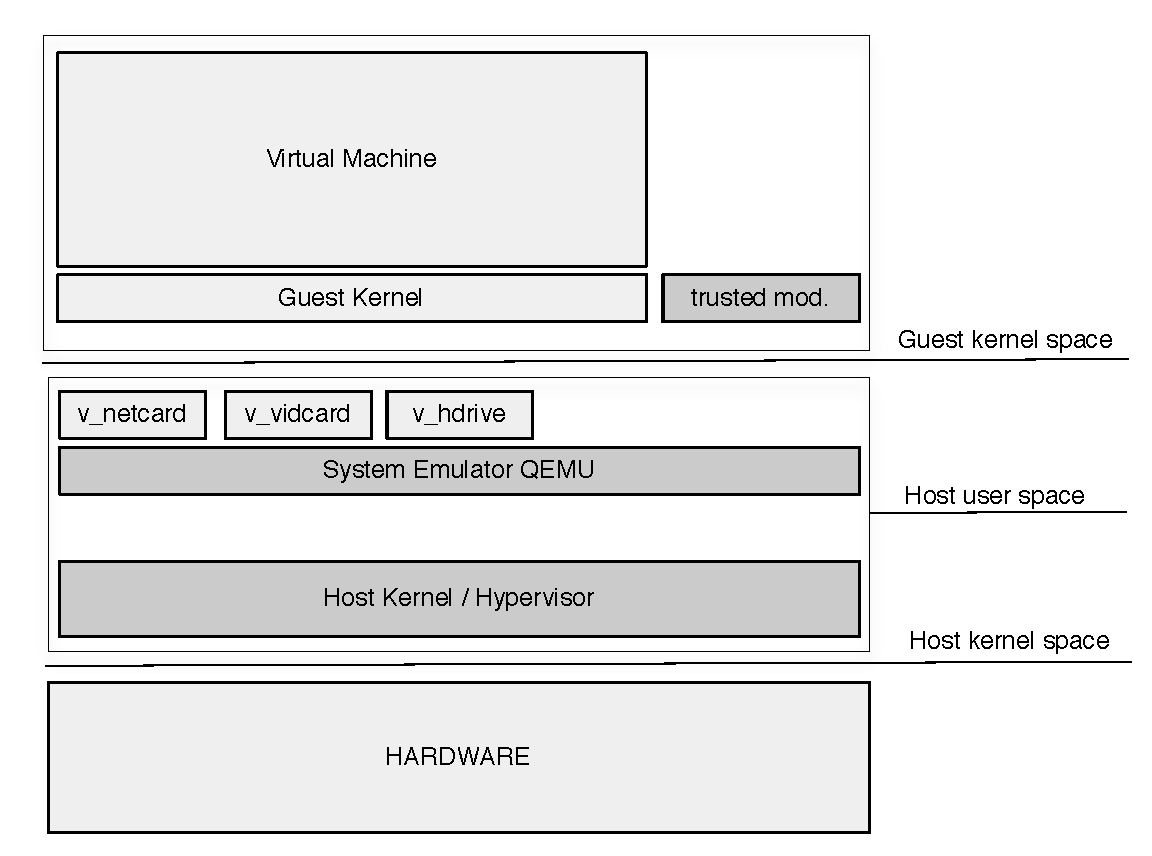
\includegraphics[scale=0.5]{images/hellorootkitty_schema.pdf}
\caption{Schema of in-hypervisor approach implemented in Linux KVM. Highlighted components indicate parts of the system that need instrumentation/modification}
\label{hellorootkitty_schema}
\end{center}
\end{figure}


Results of macro and micro-benchmarks have been collected from the guest and from the host machine and an explanation of these is given in Section \ref{macrobench} and Section \ref{microbench}.
In order to provide reliable results, all tests have been repeated 10 times and their mean value has been reported. Experiments have been performed on a machine with the hardware specification reported in Table \ref{machinespecs}.

%
%%Discussion about benchmarks (common to host and guest, micro and macro) Description of host/guest machine and environment. Performance benchmarks HyperForce  vs. hellorootKitty(KVM) According to the implementation of hello rootkitty, if the vm is not doing anything, the countermeasure is barely executed since there are very few mov cr, task switches and in general less activity. When the benchmark is executed from within the guest, this is not a problem. But when the benchmark is executed from the host we needed to stress the VM in order to force it to generate events that would have been trapped by the hypervisor. For a fair comparison with HyperForce, we stress the virtual machine in the same way and then measure the overhead of JIV from the host too.
%%Comparison with hellorootkitty:  KVM exits more frequently than Bitvisor. KVM exits also from userspace in order to give a smoother experience to the user, specially for desktop and multimedia. In order to maintain design as closer as possible to the former version of hello rootkitty we perform the checking only if a VM-Exit occured from guest kernel space.


\begin{table}[t]
\centering
\subfigure[In-host measurements]{
\label{hostmacro}
\begin{tabular}{| l | l | l |}
\hline
     ~                 & iperf [Gb/s] & overhead \\
\hline
 &  & \\
in-hyper      & 6.36         &	-               \\
HF		& 6.29         &	+1.1\%    \\
\hline
\end{tabular}
}
%\hspace{3cm}
\subfigure[In-guest measurements]{
\label{guestmacro}
\begin{tabular}{| l | l | l |}
\hline
     ~                 & iperf [Gb/s] & bunzip [sec] \\
\hline
native KVM	& 5.97       &	32.04        \\
\hline
in-hyper      & 5.26   (+12\%)      &	33.73  (+5\%)       \\
HF		& 5.71   (+4.3\%)      &	32.88  (+2.5\%)    \\
\hline
\end{tabular}
}
\caption{Macro benchmarks (\textit{in-host} OS and \textit{in-guest} OS) evaluating the integrity checking method implemented with and without HyperForce}
\label{macrobenchmarks}
\end{table}

%
\begin{comment}
\begin{table}[htdp]
\caption{Macro benchmarks (iperf -P 50 -t 300) of HyperForce (in-guest aproach) against in-hypervisor approach, within host machine}
\begin{center}
\begin{tabular}{| l | l | l | l |}
\hline
     ~                 & iperf [Gb/s] & overhead \\
\hline
in-hyper      & 6.36         &	-               \\
HF		& 6.29         &	+1.1\%    \\
\hline
\end{tabular}
\end{center}
%\label{hostmacro}
\end{table}%



\begin{table}[htdp]
\caption{Macro benchmarks of in-hypervisor approach and HyperForce, measured from the guest machine, compared to native KVM}
\begin{center}
\begin{tabular}{| l | l | l | l |}
\hline
     ~                 & iperf [Gb/s] & bunzip [sec] \\
\hline
native KVM	& 5.97       &	32.04        \\
\hline
in-hyper      & 5.26   (+12\%)      &	33.73  (+5\%)       \\
HF		& 5.71   (+4.3\%)      &	32.88  (+2.5\%)    \\
\hline
\end{tabular}
\end{center}
%\label{guestmacro}
\end{table}%
\end{comment}



\paragraph{Macro-benchmarks} \label{macrobench}
We run two macro benchmarks with the \emph{iperf} utility, that measures TCP and UDP bandwidth performance and \emph{bunzip} that extracts the Linux kernel source code from a compressed file. The original in-hypervisor version of the integrity checking method is denoted as \texttt{in-hyper} while the version using the HyperForce framework is denoted as \texttt{HF}.

While the in-hypervisor approach, due to the slower context switching, has a slightly better throughput of network performance in the host machine
Table~\ref{macrobenchmarks}(a), benchmarks in the guest machine show a considerably better performance with HyperForce.   
\emph{iperf} and \emph{bunzip} have also been executed on a native KVM system and compared against the same system running in-hypervisor and then in HyperForce. 
The performance overhead of our approach is about half of the in-hypervisor approach, as shown in Table~\ref{macrobenchmarks}(b). The original approach implemented using HyperForce performs with 4.3\% overhead compared to a native KVM guest while when implemented within hypervisor shows 12\% overhead.
The second column reports overhead of \textit{bunzip} measured in seconds. Again, HyperForce outperforms the in-hypervisor approach, showing an overhead of only 2.5\% compared to the native KVM guest.
  

\paragraph{Micro-benchmarks} \label{microbench}
Micro benchmarks show a more detailed picture of the two approaches. 
We use \emph{LMbench}~\cite{lmbench-paper}\footnote{We use version 3 of
LMbench as available at \url{http://lmbench.sourceforge.net/}.} to measure the overhead of operating system specific events such as context switch, memory mapping latency, page fault, signal handling and fork latency.
Within the host machine, HyperForce shows substantial improvement against the in-hypervisor alternative. 
In Table~\ref{hostmicro} we report only the tests where this improvement is consistent. In all other tests the in-hypervisor approach and the one using HyperForce show negligible performance overhead. 

The picture in the guest machine shows a similar trend in which HyperForce outperforms the original in-hypervisor method in every test (Table~\ref{guestmicro}).


\begin{table}[htdp]
\caption{Overhead of kernel integrity checking using the HyperForce framework (HF) is measured against in-hypervisor alternative with LMbench micro-benchmarks within the host machine. Operations are measured in microseconds.}
\begin{center}
\begin{tabular}{| l | c | c | c | c | }
\hline
~ & ctx switch  & mmap lat  & page flt 	 & mem lat \\
\hline
in-hyper     & 2.020  &	6148	&	1.57		&114.7  \\
HF		& 1.48    &	4950	&	1.46		& 101.7 \\
\hline
speedup         &+26\% & +19\% & +7\% & +11\% \\
\hline
\end{tabular}
\end{center}
\label{hostmicro}
\end{table}%

\begin{table}[htdp]
\caption{Overhead of HyperForce is measured against in-hypervisor approach with
LMbench micro-benchmarks within the guest machine. Operations are measured in microseconds.}
\begin{center}
\begin{tabular}{| l | c | c | c | c | c | c | c | c |  }
\hline
  ~            & null call  & null IO & open/close & sig inst   \\  
\hline
in-hyper & 0.30 & 0.32 & 2.32 & 0.74   \\
HF    & 0.14 & 0.21 & 2.10 & 0.45  \\  
\hline
\bf{Speedup}      &  +53\%   & +34\%    &  +10\%    & +39\%      \\
\hline
\hline

~ & sig handl & fork proc & exec proc & ctx switch \\
\hline
in-hyper 			& 5.37 & 1923 & 4087 & 5.58 \\
HF 		& 2.60 & 1788 & 3984 & 5.00 \\

\hline
\bf{Speedup}			& +51\%    & +8\%       & +2.5\%     &  +10\% \\
\hline

\end{tabular}
\end{center}
\label{guestmicro}
\end{table}%



To interpret the results shown in Table~\ref{guestmicro}, we recall that the original in-hypervisor approach performs integrity checks whenever the guest kernel writes to a control register (\texttt{MOV\_CR*} event). 
%When virtual addressing is enabled, the upper 20 bits of control register 3 (\texttt{CR3}) become the
%page directory base register, which is used to locate the page directory and
%page table of the current process. Thus, on every context switch or system
%call invocation, CR3 is modified. Trapping these events strategically
%contributes to \HRK's short attack detection time. Yet, the integrity
%checks performed by \HRK{} increase the latency of context switches and
%system calls.
%
In contrast, the implementation within the HyperForce framework employs interrupt events to trigger in-guest integrity checks. This eliminates overheads with respect to switching execution context and address mapping between the hypervisor and the guest OS, while the remaining computational overhead affects guest operations more evenly. As can be seen in Table~\ref{guestmicro}, the above changes imply significant speedups on system call invocations (53\%) and context switches (10\%). Although LMbench is often considered as insufficient for evaluating system performance~\cite{lmbenchevil}, our example shows that the benchmark suite can be used to neatly distinguish the actual speedup on system call invocations (\enquote{null call}) from the impact on a particular system call execution (e.g. \enquote{open/close}).

One may think that our approach to trigger security checks through interrupts in HyperForce reduces the security of the protected system compared to the original in-hypervisor: in the latter case an attacker increases their chance of being detected with every system call raised or process switch. However for a total
of 15,000 protected kernel objects, the worst-case detection time reported in Chapter~\ref{hr:evaluation} is about 6 seconds. 
HyperForce improves on that by checking the same amount of kernel objects in less time. 
An essential difference between the two approaches is that while the original method relies on the activity of the system as a trigger that checks the integrity of protected objects, HyperForce performs the checking independently of system activity every 4 seconds. This is the time lag of HyperForce measured while checking the entire list of objects in the guest.  

Our results indicate that the HyperForce framework could be used to re-implement other in-hypervisor applications, enhancing their performance and maintaining their effectiveness.
%
%%Protection of IDTR must occur in hypervisor's space. If this check occurs in the guest a kernel rootkit might change the IDTR to point to a different Interrupt Descriptor Table and avoid execution of security code. If the IDTR is compromised, whenever the hypervisor raises an interrupt to trigger execution of security code, a different interrupt handler might be executed. Checking the integrity of IDTR within the hypervisor prevents such an attack.

%TODO DISCARD FROM HERE
%We found two security measures that, if implemented within the Hyperforce framework, can instantly benefit of a lower performance impact. We discuss an Integrity Verification Architecture (IVA) and a kernel heap buffer overlflow monitoring system in Section \ref{IVA} and Section \ref{heapoverflow} respectively.


%\subsection{Integrity verification architecture} \label{IVA}
%\cite{isa2012integrity}
%http://www.scribd.com/doc/105446736/Integrity-Verification-Architecture-IVA-Based-Security-Framework-for-Windows-Operating-System
%we discuss an implementation of Trusted Computing in providing a mechanism to check whether hardware, software or application running on a platform “behaves as expected” without need for further validation.







%Using the Hyperforce framework will result in keeping both the monitor process and the heap buffer metadata within the target virtual machine, which in turn will reduce the overall performance impact. To ensure the same efficiency as in-the-box moni- toring, we introduce the Direct Memory Mapping (DMM) technique, which allows the monitor process to access the monitored OS memory efficiently. To protect the heap metadata and interposition code from being compromised by attackers, we apply the SIM [50] framework SIM needs to install hooks in the target kernel. 


%TODO how do we address protection of memory area in multicore systems?


\clearpage

\section{Related work}\label{hf:related}
In this section we review related work in the domain of kernel code integrity assurance. We identify three main areas of active research. Two methods that, similarly to the approach described above, inject security agents within a target system are described in Section \ref{secagent}. Protection of commodity operating systems by secure code that is isolated exploiting the hardware capabilities of modern processor architecures, is described in Section \ref{hwbased}. Finally, work related to formal verification of commodity operating systems and hypervisors is provided in Section \ref{formal}.

%For a discussion of literature related to rootkit detection we refer the reader to \cite{hellorootkitty}. 

%\paragraph{Hardware-Based Execution Flow Integrity.} Means of guaranteeing
%the integrity of a running operating system that employ dedicated hardware
%devices to monitor the physical memory of a computer system have been
%proposed in \cite{gibraltar} and \cite{copilot}. In order to perform
%integrity checks, both systems make use of PCI hardware that directly
%accesses the computer's memory at a negligible performance overhead. Yet,
%the need for dedicated hardware may hinder widespread deployment of these
%techniques.
%
%% -------------------------------------------------------------------------

%\paragraph{Hypervisor-Based Execution Flow Integrity.} 
%A tiny hypervisor that protects legacy OSs by ensuring that only validated code can be executed in kernel mode, is SecVisor~\cite{SecVisor}. 

%HyperForce can be utilized to effectively protect the integrity of the
%in-guest components of systems such as HookScout and HookSafe. Our
%experimental results obtained from implementing \HRK~\cite{hellorootkitty}
%in HyperForce show that our technique leverages the use of in-guest
%protection mechanisms. That is, HyperForce substantially reduces the
%performance overhead that would occur if the countermeasure would be
%implemented in-hypervisor, while strong security guarantees are maintained.

 
\subsection{Security Agent Injection} \label{secagent}
Closely related to the approach described in this chapter is
work by Lee et al.~\cite{lee:agent-injection} and Chiueh et al.~\cite{chiueh:sade} 
on deploying agents by means of code injection from a hypervisor. Both approaches 
are applicable to guest operating systems that have not been previously prepared by loading a 
special driver or similar.
%
In \cite{lee:agent-injection}, Lee et al. proposes to protect agent code that is 
executing in a compromised guest OS kernel by the use of cryptography and by injecting 
this code on demand from the hypervisor. As there is no implementation and no 
experimental evaluation given, a comparison with our solution is not feasible.
%
\paragraph{SADE}
Similarly, work on SADE~\cite{chiueh:sade} by Chiueh et al. uses VMWare's ESX server 
API to inject and execute code in a guest OS so as to disable and remove a previously 
detected malware infection from that guest. In difference to the HyperForce approach, 
the agent code in SADE is not protected from malicious interference on the guest. 
Chiueh et al. argue that on-demand injection leaves a relatively short time span for 
such interference. SADE is used by a virtual appliance that implements out-of-guest 
monitoring of VMs' memory, scanning for malware signatures.
The paper presents experimental data on the code injection process but does not discuss 
the overhead implied by mapping memory pages between the virtual appliance and the VMs. 
We expect in-guest memory inspection, as implemented by our kernel integrity detection 
method in HyperForce, to outperform SADE.


\paragraph{Kernel heap buffer overflow monitoring}
The primary goal of Kruiser, a security countermeasure explained in \cite{heapoverflow}, consists in detecting heap based buffer overflows in kernel space. The authors argue that those countermeasures that try to detect a buffer overflow before any write operation are usually affected by considerable performance overhead. As a consequence, the monitored process will slow down consistently whenever the monitoring system is under heavy load. Other systems perform detection occasionally, for instance whenever the buffer to be protected is deallocated. This strategy usually allows the attacker to compromise the system relatively easily, due to the large time window between corruption and detection. If a buffer is deallocated much later its corruption has occurred there are no viable ways for the countermeasure to detect and interrupt any malicious intent coming from that buffer. Finally, approaches that rely on special hardware are effective but less practical for wide deployment, as we discuss in Section \ref{hardware}.

Therefore, due to the challenging nature of protecting operating system kernels, the authors take advantage of virtualisation technology.  
The high-level idea of Kruiser consists in placing canaries into kernel heap buffers and lately check their integrity. When a canary is found to be tampered, an alarm, indicating the detection of an overflow, is raised.
In order to guarantee isolation between the monitoring and target systems, a separate process, running concurrently with the kernel, performs the checking of the canaries. 
While canaries are attached at the end of each heap buffer via an in-guest interposition mechanism, the task of  checking their integrity is decoupled and it is performed by a process running in a separate virtual machine.  
This is an essential requirement to strengthen self protection.

We argue that using the Hyperforce framework in such a scenario would allow the execution of the integrity checking process inside the guest, with native performance and without the requirements of allocating resources for any additional virtual machine. 
The hypervisor can be instructed from the trusted module about the checking frequency and the physical memory address of the protected area where canaries will be stored at runtime. The non-maskable interrupt mechanism of Hyperforce, triggered by the virtual PCI device installed within the guest, will ensure that there are no chances for the attacker to interfere with the security measure. 

As a result, Kruiser implemented in Hyperforce would become a security countermeasure that executes entirely in the target kernel, still keeping the same degree of security of the equivalent out-of-guest approach.


\subsection{Hardware-based techniques} \label{hwbased}
\paragraph{Flicker}
An infrastructure that allows the execution of security critical code, in complete isolation from the rest of the system is described in \cite{flicker}. In order to guarantee such isolation, Flicker takes advantage of hardware support such as AMD SVM or the equivalent Intel Trustes eXecution Technology. These chips allow the launch of a virtual machine monitor or a security kernel at any time, still protecting their code from malicious software.
Contrarily to hypervisor's development, that even in the case of minimal hypervisors, usually adds thousands of lines of code to the trusted computing base (TCB), the TCB of Flicker is as small as 250 lines of code. The programmer can add only the code that implements her particular application in a bottom-up approach. 
One of the most advantageous peculiarities of Flicker consists in the fact that isolation and code attestation can be guaranteed even in the presence of compromised BIOS, DMA devices and the operating system. 
When the processor receives an init instruction, it disables DMA, system interrupts and debugging access, enters at 32-bit protected mode and jumps to the provided entry point to start the execution of the isolated application.
There is no possibility for others software executing before Flicker to monitor or interfere with Flicker's code.
An example that sheds light on the potential of the aforementioned isolation property consists in a piece of code that handles a user's password, that will stay isolated from all other software running on the same machine. In the same scenario, the hardware can guarantee that the secrecy of the password has been preserved.  
The authors implemented a rootkit detector in the Flicker architecture. In this other scenario, the hardware can guarantee that no other software, the rootkit included, could tamper with the detection code. 
Any piece of code that needs to be executed in isolation should be included in a Piece of Application Logic (PAL). A Flicker session will then be initialised to begin execution of the Secure Loader Block (SLB). At the end of PAL's execution, a cleanup procedure will erase its secret values and control will return to the operating system or other untrusted components. 
Flicker offers strong security and isolation properties. But current hardware performance offered by commodity processors is not enough to consider this architecture for every day computing. 



\paragraph{TrustVisor}
Another work aimed at providing the same goals of Flicker with reduced performance penalty is TrustVisor \cite{TrustVisor}.
TrustVisor is a specially crafted hypervisor, designed to provide code and data integrity, secrecy of portions of an application (PAL) in isolation from a legacy untrusted operating system and DMA-capable devices.
The granularity of the protected code is as fine as in Flicker, although the code base is one order of magnitude higher, but still small compared to general-purpose hypervisors.
The two main capabilities of TrustVisor that use the trusted computing mechanisms offered by AMD and Intel are sealed storage and remote attestation. The former allows a particular Piece of Application Logic to encrypt data according to a policy such that the ciphertext can only be decrypted by the PAL specified in the policy. The latter is the mechanism that allows a remote party to be guaranteed that a particular PAL ran on a specific platform protected by TrustVisor.
TrustVisor can operate in host mode, which is the highest privilege level that controls hardware devices; legacy guest mode, where a commodity x86 operating system and its applications usually execute; secure guest mode, dedicated to the execution of PALs in an isolated environment.
The TrustVisor architecture is implemented taking advantage of hardware virtualisation support, in order to provide memory isolation and DMA protection for each PAL. The virtualisation mechanisms are also used by TrustVisor to protect its own code. Specifically, TrustVisor virtualises the guest operating system's memory using Nested Page Tables (NPT) and IOMMU to prevent DMA-capable devices to access arbitrary physical memory addresses.
PALs are isolated from each other with the same memory virtualisation mechanisms.
The execution of PALs follows a registration event that must be requested explicitely by the developer. Both registration and unregistration are implemented by using a hypercall that is intercepted and handled directly by TrustVisor.
The performance penalty of TrustVisor is much smaller than the one of Flicker and the security guarantees are comparable. The code base, around 6000 lines of code, is small enough to verify TrustVisor implementation using software model checking methods, that is what authors plan to achieve in the future.



\paragraph{Fides}
The goal of Fides \cite{fides} is to protect trusted modules from malware capable of exploiting vulnerabilities in the surrounding components of an operating system. The isolation properties of Fides make a vulnerable module exploitable only if other modules explicitly place trust in the former. In all other cases in which, for instance an attacker introduces malicious modules that are disconnected from the rest of the system, as is the case of rootkits, there are no viable ways to compromise the entire operating system. 
Fides combines a run-time security architecture that protects fine-grained software modules within a commodity operating system and a compiler that compiles modules written in the C language to exploit the security capabilities of the architecture on which they will execute.
The software components that execute in isolation from the rest of the system are called Self Protecting Modules (SPM). They are basically a chunk of memory, formed by a secret section, that contains the module's sensitive data and a public section that contains information for which only integrity must be guaranteed. 
The three main components that form Fides are: the legacy kernel with its applications that run without interruption and intervention of the security system; the hypervisor that manages the hardware and provides coarse grained memory isolation of the legacy and the secure virtual machines; the security kernel that manages the isolated software entities (SPM). The legacy kernel and the security kernel execute respectively in two virtual machines. Isolation and scheduling of the virtual machines are performed by the hypervisor, as in a regular virtualisation system.
The isolation among SPMs is guaranteed by the security kernel. When a module is invoked, the security kernel receives a request in which the virtual address of the entry point of the module is specified. This address is translated to its physical equivalent with the aid of Nested Paging (NPT) in the legacy virtual machine.
According to the Fides architecture, when the processor is executing outside the boundaries of the SPM, it has limited access to the module's memory. Also the destruction of the SPM follows a protocol that will leave no trace of its secret values to other components. 
SPM modules can be written in C and compiled with a modified version of LLVM, that the authors provide. The aforementioned compiler ensures that each module implements its own stack, that registers and other sensitive areas are cleared upon returning to unprotected memory, that function pointers point to unprotected memory or to a function within an SPM correctly signed, and other security measures to execute in the Fides architecture.
The overall performance impact has been measured to 3.22\%, but for applications that make heavy usage of SPMs it can grow up to 14\%.
The abilities of Fides such as confidentiality and integrity of module data, authentication and secure communication between modules, makes this architecture a suitable solution for high security environments.


\paragraph{P-maps}
The observations of the authors of P-MAPS \cite{pmaps} consist in the fact that stealthy malware can easily take advantage of the complexity of commodity operating systems. Moreover anti malware signature-based systems do not sufficiently protect against new malware, since they can recognise only known signatures. P-MAPS is a processor-measured service layer that reduces the trusted computing base of the target system in a dynamic way. This in turn improves the runtime security of user's applications without interrupting the regular execution of the operating system. P-MAPS has been designed to minimise its footprint so that it can be considered to protect mobile platforms, in which hardware and battery life are limited resources.
Moreover, according to P-MAPS authors, the existing programming model should not be changed, low performance impact should be guaranteed when protection is active and there might be the co-existence with other hardware-based security countermeasures.
The threat vector that the authors of P-MAPS address include internet downloads, an important source of malicious software downloaded in the form of system utilities, video codecs, etc, buffer overflows, still an effective and common practice to trigger attacks, network based infections such as via instant messages, peer-to-peer applications or emails. The type of attacks that can be prevented by P-MAPS are code tampering, unauthorised data access, screen scraping, key logging, man-in-the-middle, Denial Of Service, to name a few.
From a hardware view point, P-MAPS takes advantage of the virtualisation capabilities of Intel processors and Intel TXT.
The architecture of P-MAPS is straightforward. P-MAPS core executes in the highest privilege level mode (VMX root) by which hardware separation from the target application is guaranteed. The P-MAPS core isolates the program's memory from other software executing on the platform, including the operating system kernel. Moreover in this architecture only code that is stored in the measured application pages can access application data and the circumvention of a function entry point exposed by a shared library is prohibited. 
The platform starts with a commodity operating system running directly on physical hardware. As the P-MAPS protected application is launched, the P-MAPS core is loaded, measured and installed by the processor. Intel TXT technology is used to launch a trusted software environment at any time without platform reset (this is called late launch). At this point the application starts in untrusted mode and, once measured and protected by the P-MAPS core it executes in protected mode. The operating system executes in VMX-non root mode, as a guest. When the application terminates the P-MAPS core is uninstalled and the operating system is executed back on physical hardware.
Although all the security and isolation requirements are fulfilled within the P-MAPS architecture, switching between the two environments has a large performance impact. 


%\paragraph{Integrity verification architecture (IVA)} \label{IVA}
%\cite{isa2012integrity}
%http://www.scribd.com/doc/105446736/Integrity-Verification-Architecture-IVA-Based-Security-Framework-for-Windows-Operating-System
%we discuss an implementation of Trusted Computing in providing a mechanism to check whether hardware, software or application running on a platform “behaves as expected” without need for further validation. The purpose of IVA is to increase useensuring integrity of the Windows OS is astate. This means monitoring the integricomponents such as system files, registry iapplication files that run in the client platform

\subsection{Formally verified systems} \label{formal}
Formally verifying software means that it becomes possible to guarantee the absence of bugs and, taking security even further, to predict exactly how the verified piece of software will behave under any condition. Formal verification has always been an appealing goal for security researchers since, in theory, it can lead to operating system kernels that never crash and that will never perform unsafe operations \cite{Elphinstone}.  

The verification process takes place in the form of a mathematical proof that the software to be verified is bug-free and consistent with its specification \cite{formalpractice}.
Unfortunately, the complexity of the verification, the code size of commodity operating systems and the complexity of the hardware mechanisms on which they are executed, make the complete verification of such systems more an illusion rather than a goal that can be achieved in the immediate future. 
However, consistent simplifications and initial assumptions can make the task of verification slightly easier. 

In light of virtualisation technology, seeking for a formal verification of hypervisors makes more sense than verifying the single guest operating systems because 1) hypervisors have a much simpler architecture than commodity operating systems and 2) the hypervisor is becoming the bottleneck of a virtualisation platform in terms of performance and security. 
In order to shed light on the two different fields in which formal verification practitioners have to deal with, we report a formal verification of a simplified operating system and two studies conducted towards the verification of a hypervisor.

\paragraph{seL4}
The first formal proof of functional correctness of a general-purpose operating system kernel is achieved by \cite{sel4}. The authors provide a machine-checked verification of the seL4 microkernel from an abstract specification to its implementation in the C programming language.
Correctness of the compiler, assembly code and hardware are some of the assumptions that anticipate the formal proof. Although the seL4 kernel is directly usable on ARMv6 and x86 architectures, a proof on the latter is missing. The model assumes that all memory allocations occurring in the kernel are explicit and authorised.
While operating system development follows a bottom-up approach to kernel design, formal verification practitioners have the tendency to verify in a top-down fashion, in order to control the level of complexity of the overall system. seL4 is verified using an approach that is somewhere in between the two extremes. The functional programming language Haskell is used to provide a programming interface for operating system developers and, at the same time, provide code that can be translated directly into the theorem proving tool.
The technique used to formally verifying the microkernel is interactive, namely it needs human intervention.
Each unit of proof has a set of preconditions that must hold prior to execution and a set of post-conditions that must hold afterwards. The level of complexity depends on the statement being verified. Strong simplifications are required to lower the difficulty of the verification process. Many of them do not apply to operating systems that are commonly used.
Proofs about concurrent systems are extremely hard. The authors do not consider verification of their kernel executing on multiprocessor systems. Moreover the complexity of interrupts, in the form of non-deterministic execution of handlers and preemption, is \emph{solved} by disabling interrupts most of the time except in a small number of interrupt points. Although exceptions occur synchronously, their effects are similar to the ones of interrupts. Exceptions are avoided completely in the verification of seL4. 
Due to the aforementioned oversimplifications, it is hard to believe that commodity operating systems that  executes on architectures like x86, will be formally verified soon.
   


\paragraph{Hyper-V}
One of the first attempts to verify an hypervisor has been conducted in \cite{verifyhyperv} on the Microsoft Hyper-V hypervisor. Hyper-V is relatively small and runs directly on x64 hardware. The code is divided in the \emph{kernel stratum} that includes a minimal operating system, a hardware abstraction layer, the kernel, the memory manager and the scheduler (device drivers are not included) and the \emph{virtualisation stratum}, that simulates the x64 machine for the guest operating systems. The hypervisor is written in C, which has a weak type system. But the main challenge in verifying such a piece of code is due to the presence of assembly code snippets, which leads to an integrated verification of the two languages. 
The authors use VCC, an industrial-strength verification suite that specifically addresses the formal verification of low-level C code.
Due to the static modular analysis that VCC can perform, each function is verified in isolation. Moreover, before the verification process, the original codebase is annotated. One of the authors' goals is to let these annotations evolve with the core development and to maintain them within the codebase. 
An interesting stratagem to tackle with the problem of verifying programs that deal with shared knowledge (e.g. a program that is acquiring a spin lock should know that the spin lock has been initialised and it still exists) consists in using ghost objects, called \emph{claims}, rather then preconditions. Claims are associated with many objects and they guarantee, among other properties, that the objects stay allocated as long as a claim to them exists. Ghost data and code are visible only to the verifier.
The verification chain consists in translating the code with annotations into the Boogie language, then the Boogie tool generates the verification conditions to be passed to the theorem prover.
The model of the processor core is entirely implemented with ghost functions. Specific ghost functions specify the effects of executing single x64 instructions.  The aforementioned model is used to provide verification of assembly code and to prove that Hyper-V simulates x64 instructions correctly for the guest operating systems.
Despite the relatively small codebase size of Hyper-V and the expected complexity of the verification process, the authors argue that several hundred functions have been verified and that the VCC-based approach is powerful enough to verify them all.

%The Hypervisor is part of a released product with very low defect density. Therefore, we did not expect to find many bugs in the code, and indeed less than a handful have been found during the verification process. All of them are very unlikely to let the Hy- pervisor fail in practical operation. 

\paragraph{Verification of a small hypervisor}
A work that follows to the verification of Hyper-V is presented in \cite{autoverification}. It describes the verification of a small hypervisor using VCC modeling of software-hardware interactions and simulation proofs in first-order logic. The hypervisor is a simple piece of software that simulates VAMP, a simple 32-bit RISC hardware architecture with 44 instructions and two privilege levels. In the overall modeling, single-level address translations without TLB and interrupt handling are considered. The guest operating systems are always run on the host in user mode, regardless of the mode the guests think to be executing in. This gives full control over the guests and any privilege operation can be trapped safely.
The overall work is composed by the VAMP specification and simulation, the hypervisor implementation and system programs. The authors addressed extensions both on the software side, in the form of preemptive kernels and software parallelism, and on the hardware side, in the form of multi-core systems, hardware buffers like the TLB and devices. Part of these extensions are ongoing work.


\paragraph{Xenon}
A more recent attempt to formally verify a widely used hypervisor like Xen \cite{xen} is Xenon \cite{xenon}. In the aforementioned work a formal security policy model is defined, starting from the original version of the Xen hypervisor. The authors argue they provide a robust information flow control, tamper-resistance and self- protection of the virtual machines (called execution environments) running on top of their hypervisor. 
Their basic approach consists in confining each user community in its own execution environment and limiting the information flow between two environments to a restricted form of replication. Namely, an execution environment that is reading data from another environment, will get access to a local copy of the data.
The policy that allows or denies information flow between two execution environments is called \emph{security domain lattice}. 
The Xenon formal security model is written in CSP, an algebra to model non-interference and other trace-based information flow security policies. Moreover, CSP is well suited for reasoning about communication patterns between multiple threads of computation. These patterns are defined as sets of traces of instantaneous events and their duration is not modelled. 
The Xenon model has been decomposed in subsystems that are modelled separately. Three subsystems have been identified, namely the boundary controller, the guest process and the virtual machine monitor process. The complete model that results from the parallel combination of the guest and the virtual machine monitor is deadlock free.
Some peculiarities of the Xenon model consist in the fact that hypercalls, interrupts, traps, privileged and unprivileged instructions are considered Xenon events. Moreover the virtual machine monitor interface provides data structures such as virtual memory, virtual machine control structures (VMSC) and device driver front ends the effects of which can be mapped as Xenon events.
Processes are used to model data structures, as a conventional CSP technique. When data have been transformed into CSP processes, the overall complexity of the verification process is reduced because it is possible to interchangeably refer to the interface data structures as though they were processes.
Although the formal model does not support non-deterministic interrupts, a simplification represents them as signal events that arise deterministically within the virtual machine monitor. 
Due to the structure of the policy model that results close to the structure of an implementation, the authors of Xenon argue that they will implement it on 64-bit x86 architecture.



\section{Summary}\label{hf:conclusion}
%The attractive properties offered by virtualization are a foundational
%block for the whole ``cloud technology''. At the same time, virtualization
%is already being used for purposes other than the deployment of multiple
%operating systems as a way of increasing the security of a single
%virtualized operating system. 
In this chapter we briefly discuss the differences between security mechanisms 
deployed within an operating system (\textit{in-guest}) and the ones deployed 
within a hypervisor (\textit{in-hypervisor}) and bring attention to the, 
seemingly exclusive, choice between the performance benefits of the former 
versus the security benefits of the latter. 

We tackle this choice by developing a hybrid framework, allowing security mechanisms 
to be developed in a way that provides them with performance analogous to \textit{in-guest} 
systems while maintaining the security of \textit{in-hypervisor} systems. 

Using this new concept, we re-implemented an \textit{in-hypervisor} rootkit detection
system and show how the new version significantly outperforms the original
without compromising the security or integrity of the detection system.

We conclude that hybrid security systems that are built on top of the described 
framework can provide effective and efficient alternatives to mitigate the
overhead of techniques that exclusively operate in-hypervisor.
An interesting type of applications that might be designed with our framework in mind, is represented by malware
detection and removal software, for which both isolation from the target system and 
performance must be guaranteed, in order to take full advantage of the protection capabilities that these systems usually claim.

Another constraint we tackle with consists in the size of instrumentation code required 
by our approach. We believe that smaller instrumentation code size will ease the 
adoption of that security countermeasure and facilitate its deployment within production 
systems.

%FIXME 
%For future work we envisage to extend our framework with techniques to inject 
%security agents into a guest operating system so as to provide secure means 
%of on-demand deployment of such agents.
